% !TEX TS-program = pdflatex
% PEC-E: Principle of Emergent Cycles — Full Draft with TikZ Figures
\documentclass[11pt,a4paper]{article}

% -------------------- Packages --------------------
\usepackage[T1]{fontenc}
\usepackage[utf8]{inputenc}
\usepackage{lmodern}
\usepackage[margin=2.5cm]{geometry}
\usepackage{setspace}
\usepackage{microtype}
\usepackage{authblk}
\usepackage{titlesec}
\usepackage{enumitem}
\usepackage{graphicx}
\usepackage{caption}
\usepackage{subcaption}
\usepackage{booktabs}
\usepackage{siunitx}
\usepackage{amsmath,amssymb,amsfonts,amsthm}
\usepackage{mathtools}
\usepackage{bm}
\usepackage{hyperref}
\hypersetup{colorlinks=true,linkcolor=blue,citecolor=blue,urlcolor=blue}

% TikZ / PGF
\usepackage{tikz}
\usetikzlibrary{arrows.meta,positioning,calc,fit,backgrounds,shapes,decorations.pathmorphing}
\usepackage{pgfplots}
\pgfplotsset{compat=1.18}

% -------------------- Formatting --------------------
\titleformat{\section}[hang]{\Large\bfseries}{\thesection}{0.75em}{}
\titleformat{\subsection}[hang]{\large\bfseries}{\thesubsection}{0.65em}{}
\titleformat{\subsubsection}[hang]{\normalsize\bfseries}{\thesubsubsection}{0.5em}{}

\setlist[itemize]{topsep=2pt,itemsep=2pt,leftmargin=1.5em}
\setlist[enumerate]{topsep=2pt,itemsep=2pt,leftmargin=1.7em}

\onehalfspacing

% -------------------- Title --------------------
\title{The Principle of Emergent Cycles: Entropy, Selection, and the Origins of Stability}
\author[1]{Albert Jan van Hoek}
\author[2]{\small Collaborators TBD}
\affil[1]{\small Public Health Sciences, Hilversum, NL}
\affil[2]{\small Institution(s) TBD}
\date{Draft: September 23, 2025}

% -------------------- Macros --------------------
\newcommand{\EE}{\mathrm{E}}
\newcommand{\PP}{\mathrm{P}}
\newcommand{\dd}{\mathrm{d}}
\newcommand{\dotS}{\dot S_{\mathrm{tot}}}
\newcommand{\phifrac}{\phi}
\newcommand{\comp}{\mathrm{Comp}}
\newcommand{\stab}{\mathrm{Stab}}
\newcommand{\Eset}{\mathcal{E}}
\newcommand{\Cset}{\mathcal{C}}

% -------------------- Document --------------------
\begin{document}
\maketitle

\begin{abstract}
We propose the \emph{Principle of Emergent Cycles (PEC-E)}: in open, driven, non-equilibrium systems, dissipation organizes into recurrent cycles, but only a rare subset of cycles persists. Emergent cycles are selected because they simultaneously channel entropy (increasing the cycle-carried fraction \(\phifrac\)), stabilize dynamics (shorter return times, lower variance), and enable higher-order composition (new loops on top of stable ones). This refines naive claims that ``more feedback yields stability'' by acknowledging that random complexity often destabilizes. Instead, PEC-E identifies emergence as a pruning process: entropy generates variation, unstable loops collapse, and rare stable loops remain and scaffold further organization. We formalize PEC-E with a fitness functional on cycles, propose falsifiable predictions, and outline an empirical program across chemical, biological, ecological, and engineered systems.
\end{abstract}

\section{Introduction}
The Second Law guarantees that entropy increases, yet it does not specify the \emph{organization} of dissipation. Nevertheless, far-from-equilibrium systems frequently settle into \emph{recurrent} structures: convection rolls, autocatalytic loops, metabolic cycles, physiological and ecological feedbacks. Why do \emph{cycles} emerge, and why do they persist? The classical expectation that complexity yields stability has been challenged by results showing that random increases in interaction density destabilize ecosystems and that excessive feedback can cause oscillations or collapse in physiology and engineered systems. Yet nature abounds with \emph{stable} cycles. We argue that \emph{emergence as pruning} resolves this paradox.

\paragraph{Thesis (PEC-E).} Under sustained drive and perturbation, dissipation tends to explore many cyclic pathways; a \emph{rare} subset persists because these cycles both (i) channel entropy productively and (ii) stabilize the larger network while (iii) enabling further composition. Emergence is this selection-and-persistence of stabilizing loops.

\paragraph{Reflexive note.} This work is itself an emergent loop. We know complexity exists because we exist; in asking how it persists, we generate new structures (definitions, models, predictions) that in turn stabilize our understanding and allow further questions. In the spirit of PEC-E, the paper proposes a sparse backbone of concepts—\emph{dissipation, cycles, pruning, composition} -around which later refinements can accrete. The search is the finding: the theory organizes its own inquiry into a persistent cycle.

\section{Background}
\subsection{Cycles and entropy production}
In continuous-time Markov processes (master equations), Schnakenberg's network thermodynamics decomposes stationary total entropy production as
\begin{equation}
\dotS \,=\, \frac{1}{2}\sum_{i,j} J_{ij} A_{ij} \,=\, \sum_{\alpha} J_{\alpha} A_{\alpha},
\end{equation}
where $J_{ij}$ are edge currents and $A_{ij}$ affinities; the right-hand side sums over a cycle basis with cycle currents $J_{\alpha}$ and affinities $A_{\alpha}$. This representation motivates the \emph{cycle-carried fraction} of dissipation
\begin{equation}
\phifrac \,=\, \frac{\sum_{\alpha\in \text{nontrivial}} J_{\alpha}A_{\alpha}}{\dotS} \in [0,1].
\end{equation}

\subsection{The complexity--stability paradox}
Random complexity can destabilize: May's models show reduced stability with increasing richness and connectance; enrichment can destabilize predator--prey cycles (Rosenzweig). Engineered networks display robust-yet-fragile behavior; biological positive feedback loops (e.g., reentrant arrhythmias) can be pathological. Thus, ``more loops'' is not sufficient for stability.

\subsection{Emergence as pruning}
Real systems are not random. They exhibit \emph{selected} loops---weak ties, negative feedback, and composable modules---that survive perturbations. We reinterpret emergence as a \emph{filter} that prunes unstable cycles, leaving a sparse backbone of persistent loops.

\section{Principle of Emergent Cycles (PEC-E)}
\subsection{Operational definition}
A cycle $c$ is \emph{non-trivial} if it exhibits positive entropy production at stationarity ($J_{\alpha}A_{\alpha}>0$) and remains detectable across reasonable coarse-grainings. A cycle is \emph{emergent} if it additionally:
\begin{itemize}
  \item increases the cycle-carried fraction $\Delta\phifrac(c) > 0$ at the relevant scale;
  \item improves local stability $\Delta\stab(c) > 0$ (shorter return time, lower variance);
  \item increases composability $\Delta\comp(c) > 0$ (enables new higher-order loops);
  \item persists under noise and coarse-graining (robustness band on $\phifrac$).
\end{itemize}

\subsection{Fitness functional and emergent set}
Define
\begin{equation}
F(c) = w_1\,\Delta\phifrac(c) + w_2\,\Delta\stab(c) + w_3\,\Delta\comp(c),\qquad w_i\ge 0,
\end{equation}
with threshold $\tau$. The \emph{emergent set} is $\Eset(\Cset)=\{c\in\Cset: F(c)\ge \tau\}$.

\subsection{Predicted regimes under increasing drive}
At low drive, dissipation is mostly linear (small $\phifrac$). As drive rises, many loops appear, most unstable; pruning leaves a sparse set of emergent loops with elevated $\phifrac$ and stability. At very high drive, over-coupling can yield fragility (overshoot/oscillation).

\section{Coarse-graining and robustness}
Cycles depend on state partitioning. We adopt three safeguards: (i) \emph{natural partitions} (chemically distinct species, functional modules); (ii) \emph{robustness bands} for $\phifrac$ across partitions; (iii) \emph{trend consistency} (sign of $\partial\phifrac/\partial C$ preserved across reasonable coarse-grainings). PEC-E is supported if trends persist within bands; it fails if $\phifrac$ is arbitrary under benign coarse-graining.

\section{Predictions and falsifiability}
\paragraph{P1 (Cycle scaling).} Along complexity ramps (more feedback, catalysts), $\phifrac$ increases after pruning; unstable loops collapse.
\paragraph{P2 (Stability).} Emergent loops shorten return time and reduce variance; excessive gain induces fragility.
\paragraph{P3 (Composition).} Emergent loops increase higher-order loop formation rates.
\paragraph{Falsifiers.} (i) No $\Delta\phifrac>0$ under sustained drive+feedback; (ii) $\phifrac$ decreases with complexity post-pruning; (iii) $\phifrac$ trends flip under reasonable coarse-grainings; (iv) systems robustly prefer linear dissipation when loops are available.

\section{Case studies (sketches)}
\subsection{Cellular metabolism}
Chemostat experiments with \textsuperscript{13}C flux analysis under nutrient stress: test whether persistent cycles (e.g., TCA) carry increasing fractions of dissipation ($\phifrac$) and whether recovery improves.

\subsection{Physiology}
Baroreflex perturbations (tilt, CO\textsubscript{2}): quantify loop gain/phase and return time; relate to $\phifrac$-like metrics in control actions.

\subsection{Ecosystems}
Nutrient enrichment: expect initial oscillations (random loops), then stabilization by weak, structured loops; measure cycling indices and variance.

\subsection{Engineered systems}
Power-grid simulations: intermediate loop depth increases robustness; excessive feedback yields oscillations; map to $\phifrac$ and stability.

\section{Relation to existing principles}
\textbf{MEP.} PEC-E is orthogonal: some systems maximize entropy production, but only stabilizing loops persist. \textbf{Constructal law.} Access optimization yields branching structures; PEC-E highlights recurrent loops as persistent architecture. \textbf{Robust-yet-fragile.} PEC-E predicts fragility beyond optimal loop gain.

\section{Discussion}
PEC-E reframes cycles as the outcomes of variation and pruning: entropy generates candidates; selection retains those that stabilize and compose. This reconciles the prevalence of loops with the instability of random complexity and provides cross-scale explanatory power.

\section{Conclusion}
Entropy drives cycles; emergence selects the few that last. These emergent cycles stabilize systems and scaffold further organization. PEC-E offers falsifiable, quantitative predictions and an empirical program uniting thermodynamics, biology, ecology, and engineering.

\section*{Methods: computing \texorpdfstring{$\phifrac$}{phi} and stability}
Given a stationary Markov network with rates $k_{ij}$ and stationary distribution $\pi_i$, define currents $J_{ij}=\pi_i k_{ij}-\pi_j k_{ji}$ and affinities $A_{ij}=\ln(\pi_i k_{ij}/\pi_j k_{ji})$. Construct a cycle basis (e.g., fundamental cycles from a spanning tree). Compute cycle currents $J_\alpha$ and affinities $A_\alpha$; then $\dotS=\sum_\alpha J_\alpha A_\alpha$ and $\phifrac=\sum_{\alpha\in \text{nontrivial}} J_\alpha A_\alpha/\dotS$. Stability metrics include mean return time to a reference set, variance of observables under perturbation, and spectral gap.

% -------------------- Figures --------------------
\clearpage
\section*{Figures}

% Figure 1: phi vs drive, with regimes
\begin{figure}[h]
  \centering
  \begin{tikzpicture}[scale=1.0]
    % Axes
    \draw[->] (0,0) -- (10,0) node[below right]{Drive (gradient)};
    \draw[->] (0,0) -- (0,5) node[left]{Cycle-carried fraction $\,\phifrac$};
    % Curve (S-shaped with plateau)
    \draw[thick,domain=0:9,smooth,variable=\x] plot ({\x},{ 0.2 + 3.2/(1+exp(-0.9*(\x-4))) / 3 }) ;
    % Regime labels
    \node at (1.2,0.6) {\small Linear};
    \node at (4.0,2.2) {\small Proliferation};
    \node at (7.6,3.4) {\small Pruned plateau};
    % Braces / regions
    \draw[dashed] (3.3,0) -- (3.3,4.5);
    \draw[dashed] (6.7,0) -- (6.7,4.5);
    \node[below] at (1.6,0){\small Low drive};
    \node[below] at (5.0,0){\small Mid drive};
    \node[below] at (8.3,0){\small High drive};
  \end{tikzpicture}
  \caption{Schematic of $\phifrac$ (fraction of entropy production carried by cycles) versus drive. Low drive: mostly linear. Mid: many loops appear (unstable). After pruning: emergent loops dominate, yielding a stable band.}
\end{figure}

% Figure 2: Network diagrams (linear -> loopy -> pruned backbone)
\begin{figure}[h]
  \centering
  \begin{subfigure}[b]{0.31\textwidth}
    \centering
    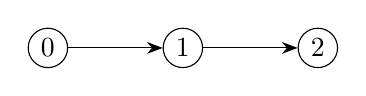
\begin{tikzpicture}[node distance=1.2cm]
      \tikzstyle{n}=[circle,draw,minimum size=5mm,inner sep=0pt]
      \node[n] (a) {0};
      \node[n,right=of a] (b) {1};
      \node[n,right=of b] (c) {2};
      \draw[-{Stealth[length=2mm]}] (a) -- (b);
      \draw[-{Stealth[length=2mm]}] (b) -- (c);
    \end{tikzpicture}
    \caption{Linear}
  \end{subfigure}\hfill
  \begin{subfigure}[b]{0.31\textwidth}
    \centering
    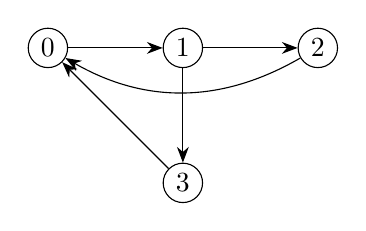
\begin{tikzpicture}[node distance=1.2cm]
      \tikzstyle{n}=[circle,draw,minimum size=5mm,inner sep=0pt]
      \node[n] (a) {0};
      \node[n,right=of a] (b) {1};
      \node[n,right=of b] (c) {2};
      \node[n,below=of b] (d) {3};
      \draw[-{Stealth[length=2mm]}] (a) -- (b);
      \draw[-{Stealth[length=2mm]}] (b) -- (c);
      \draw[-{Stealth[length=2mm]}] (b) -- (d);
      \draw[-{Stealth[length=2mm]}] (d) -- (a);
      \draw[-{Stealth[length=2mm]}] (c) edge[bend left] (a);
    \end{tikzpicture}
    \caption{Loopy (many cycles)}
  \end{subfigure}\hfill
  \begin{subfigure}[b]{0.31\textwidth}
    \centering
    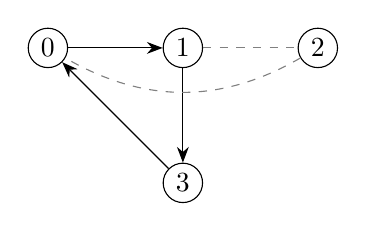
\begin{tikzpicture}[node distance=1.2cm]
      \tikzstyle{n}=[circle,draw,minimum size=5mm,inner sep=0pt]
      \node[n] (a) {0};
      \node[n,right=of a] (b) {1};
      \node[n,right=of b] (c) {2};
      \node[n,below=of b] (d) {3};
      % pruned backbone cycles
      \draw[-{Stealth[length=2mm]}] (a) -- (b);
      \draw[-{Stealth[length=2mm]}] (b) -- (d);
      \draw[-{Stealth[length=2mm]}] (d) -- (a);
      % faint removed edges
      \draw[gray,dashed] (b) -- (c);
      \draw[gray,dashed] (c) edge[bend left] (a);
    \end{tikzpicture}
    \caption{Pruned backbone}
  \end{subfigure}
  \caption{From linear dissipation to proliferation of loops, then pruning to a sparse, persistent cycle backbone (emergent cycles).}
\end{figure}

% Figure 3: Phase diagram (where PEC-E holds vs breaks)
\begin{figure}[h]
  \centering
  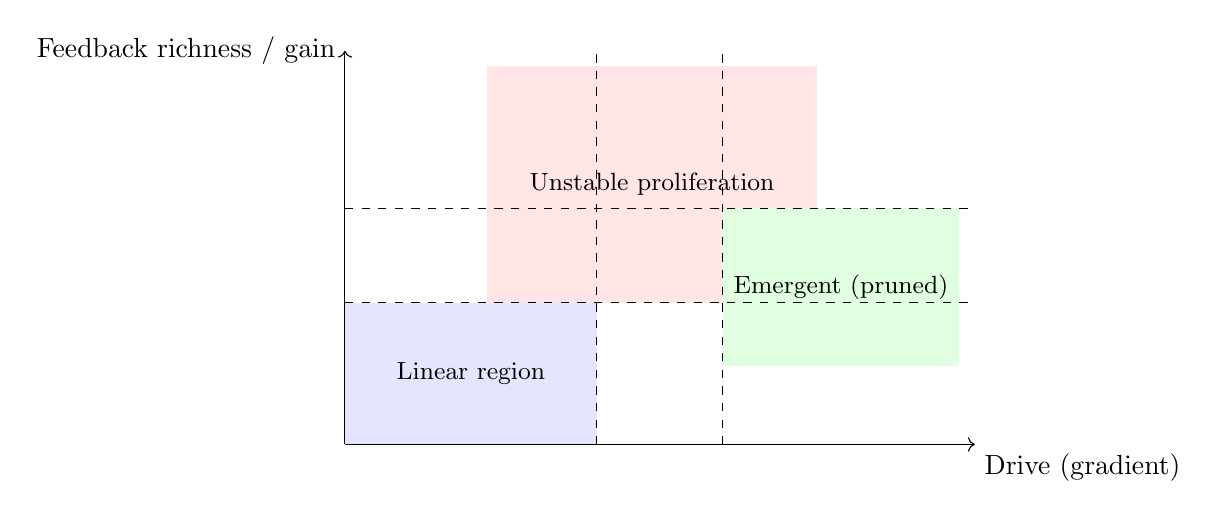
\begin{tikzpicture}[scale=1.0]
    % axes
    \draw[->] (0,0) -- (8,0) node[below right]{Drive (gradient)};
    \draw[->] (0,0) -- (0,5) node[left]{Feedback richness / gain};
    % regions
    \fill[blue!10] (0,0) rectangle (3.2,1.8);
    \node at (1.6,0.9) {\small Linear region};
    \fill[red!10] (1.8,1.8) rectangle (6.0,4.8);
    \node at (3.9,3.3) {\small Unstable proliferation};
    \fill[green!12] (4.8,1.0) rectangle (7.8,3.0);
    \node at (6.3,2.0) {\small Emergent (pruned)};
    % boundaries
    \draw[dashed] (3.2,0) -- (3.2,5);
    \draw[dashed] (0,1.8) -- (8,1.8);
    \draw[dashed] (4.8,0) -- (4.8,5);
    \draw[dashed] (0,3.0) -- (8,3.0);
  \end{tikzpicture}
  \caption{Heuristic phase diagram: at low drive/feedback, dynamics are linear; at moderate/high both, unstable loop proliferation; in a window (green), pruning yields emergent cycles and stability. Outside this window (top-right), over-coupling leads to fragility.}
\end{figure}

% Figure 4: Case study contrast (beneficial metabolic loop vs harmful reentrant loop)
\begin{figure}[h]
  \centering
  \begin{subfigure}[b]{0.48\textwidth}
    \centering
    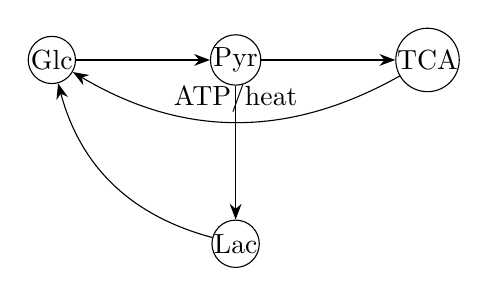
\begin{tikzpicture}[node distance=1.7cm]
      \tikzstyle{n}=[circle,draw,minimum size=6mm,inner sep=0pt]
      \node[n] (glc) {Glc};
      \node[n,right=of glc] (pyr) {Pyr};
      \node[n,right=of pyr] (tca) {TCA};
      \node[n,below=of pyr] (lac) {Lac};
      \draw[-{Stealth[length=2mm]}] (glc) -- (pyr);
      \draw[-{Stealth[length=2mm]}] (pyr) -- (tca);
      \draw[-{Stealth[length=2mm]}] (tca) edge[bend left] node[above]{ATP/heat} (glc);
      \draw[-{Stealth[length=2mm]}] (pyr) -- (lac);
      \draw[-{Stealth[length=2mm]}] (lac) edge[bend left] (glc);
    \end{tikzpicture}
    \caption{Beneficial metabolic cycling: stable, composable}
  \end{subfigure}\hfill
  \begin{subfigure}[b]{0.48\textwidth}
    \centering
    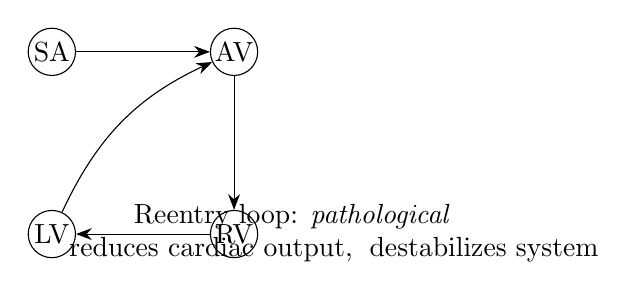
\begin{tikzpicture}[node distance=1.7cm]
      \tikzstyle{n}=[circle,draw,minimum size=6mm,inner sep=0pt]
      \node[n] (sa) {SA};
      \node[n,right=of sa] (av) {AV};
      \node[n,below=of av] (rv) {RV};
      \node[n,left=of rv] (lv) {LV};
      \draw[-{Stealth[length=2mm]}] (sa) -- (av);
      \draw[-{Stealth[length=2mm]}] (av) -- (rv);
      \draw[-{Stealth[length=2mm]}] (rv) -- (lv);
      \draw[-{Stealth[length=2mm]}] (lv) edge[bend left=20] (av);
      \node[align=center,anchor=west] at (0.1,-2.3) {Reentry loop: \textit{pathological}\,\,\,\,\,\,\,\,\,\,\,\,\,\,\,\,\,\,\\ reduces cardiac output,\; destabilizes system};
    \end{tikzpicture}
    \caption{Pathological reentrant loop: destabilizing}
  \end{subfigure}
  \caption{Not all loops stabilize. Emergent loops contribute to stability and composition (left). Others (right) are selected against or clinically suppressed.}
\end{figure}

\clearpage
\section*{References}
\begin{thebibliography}{99}
\bibitem{May1972} May, R. M. Will a Large Complex System be Stable? \emph{Nature} \textbf{238}, 413–414 (1972).
\bibitem{Rosenzweig1971} Rosenzweig, M. L. Paradox of Enrichment: Destabilization of Exploitation Ecosystems in Ecological Time. \emph{Science} \textbf{171}, 385–387 (1971).
\bibitem{Schnakenberg1976} Schnakenberg, J. Network theory of microscopic and macroscopic behavior of master equation systems. \emph{Rev. Mod. Phys.} \textbf{48}, 571–585 (1976).
\bibitem{HaldaneMay2011} Haldane, A. G. \& May, R. M. Systemic risk in banking ecosystems. \emph{Nature} \textbf{469}, 351–355 (2011).
\bibitem{Doyle2005} Doyle, J. C., Alderson, D. L., Li, L. et al. The "robust yet fragile" nature of the Internet. \emph{PNAS} \textbf{102}(41), 14497–14502 (2005).
\bibitem{DiVita2010} Di Vita, A. Maximum or minimum entropy production? \emph{Phys. Rev. E} \textbf{81}, 041137 (2010).
\end{thebibliography}

\end{document}
